% Options for packages loaded elsewhere
\PassOptionsToPackage{unicode}{hyperref}
\PassOptionsToPackage{hyphens}{url}
\documentclass[
  ignorenonframetext,
  aspectratio=169]{beamer}
\newif\ifbibliography
\usepackage{pgfpages}
\setbeamertemplate{caption}[numbered]
\setbeamertemplate{caption label separator}{: }
\setbeamercolor{caption name}{fg=normal text.fg}
\beamertemplatenavigationsymbolsempty
% remove section numbering
\setbeamertemplate{part page}{
  \centering
  \begin{beamercolorbox}[sep=16pt,center]{part title}
    \usebeamerfont{part title}\insertpart\par
  \end{beamercolorbox}
}
\setbeamertemplate{section page}{
  \centering
  \begin{beamercolorbox}[sep=12pt,center]{section title}
    \usebeamerfont{section title}\insertsection\par
  \end{beamercolorbox}
}
\setbeamertemplate{subsection page}{
  \centering
  \begin{beamercolorbox}[sep=8pt,center]{subsection title}
    \usebeamerfont{subsection title}\insertsubsection\par
  \end{beamercolorbox}
}
% Prevent slide breaks in the middle of a paragraph
\widowpenalties 1 10000
\raggedbottom
\AtBeginPart{
  \frame{\partpage}
}
\AtBeginSection{
  \ifbibliography
  \else
    \frame{\sectionpage}
  \fi
}
\AtBeginSubsection{
  \frame{\subsectionpage}
}
\usepackage{iftex}
\ifPDFTeX
  \usepackage[T1]{fontenc}
  \usepackage[utf8]{inputenc}
  \usepackage{textcomp} % provide euro and other symbols
\else % if luatex or xetex
  \usepackage{unicode-math} % this also loads fontspec
  \defaultfontfeatures{Scale=MatchLowercase}
  \defaultfontfeatures[\rmfamily]{Ligatures=TeX,Scale=1}
\fi
\usepackage{lmodern}
\usetheme[]{Madrid}
\usefonttheme[]{structurebold}
\ifPDFTeX\else
  % xetex/luatex font selection
\fi
% Use upquote if available, for straight quotes in verbatim environments
\IfFileExists{upquote.sty}{\usepackage{upquote}}{}
\IfFileExists{microtype.sty}{% use microtype if available
  \usepackage[]{microtype}
  \UseMicrotypeSet[protrusion]{basicmath} % disable protrusion for tt fonts
}{}
\makeatletter
\@ifundefined{KOMAClassName}{% if non-KOMA class
  \IfFileExists{parskip.sty}{%
    \usepackage{parskip}
  }{% else
    \setlength{\parindent}{0pt}
    \setlength{\parskip}{6pt plus 2pt minus 1pt}}
}{% if KOMA class
  \KOMAoptions{parskip=half}}
\makeatother
\usepackage{longtable,booktabs,array}
\usepackage{calc} % for calculating minipage widths
\usepackage{caption}
% Make caption package work with longtable
\makeatletter
\def\fnum@table{\tablename~\thetable}
\makeatother
\setlength{\emergencystretch}{3em} % prevent overfull lines
\providecommand{\tightlist}{%
  \setlength{\itemsep}{0pt}\setlength{\parskip}{0pt}}
\setbeamertemplate{footline}{}
\setbeamertemplate{navigation symbols}{}
\definecolor{RoadYellow}{RGB}{242,204,0}
\definecolor{RoadBlack}{RGB}{20,20,20}
\definecolor{RoadGray}{RGB}{245,245,245}
\setbeamercolor{palette primary}{bg=RoadBlack, fg=RoadYellow}
\setbeamercolor{palette secondary}{bg=RoadBlack, fg=white}
\setbeamercolor{palette tertiary}{bg=RoadYellow, fg=RoadBlack}
\setbeamercolor{palette quaternary}{bg=RoadBlack, fg=white}
\setbeamercolor{structure}{fg=RoadYellow}
\setbeamercolor{title}{fg=RoadYellow}
\setbeamercolor{frametitle}{bg=RoadBlack, fg=RoadYellow}
\setbeamercolor{normal text}{fg=black, bg=white}
\setbeamercolor{block title}{bg=RoadBlack, fg=RoadYellow}
\setbeamercolor{block body}{bg=RoadGray, fg=black}
\setbeamercolor{item}{fg=RoadYellow}
\setbeamertemplate{footline}{}
\setbeamertemplate{navigation symbols}{}
\usepackage{bookmark}
\IfFileExists{xurl.sty}{\usepackage{xurl}}{} % add URL line breaks if available
\urlstyle{same}
\hypersetup{
  pdftitle={Are Harris County Drivers the Worst in Texas?},
  pdfauthor={Fredy Guevara},
  hidelinks,
  pdfcreator={LaTeX via pandoc}}

\title{Are Harris County Drivers the Worst in Texas?}
\subtitle{An Editable Beamer Presentation}
\author{Fredy Guevara}
\date{2026-04-14}

\begin{document}
\frame{\titlepage}

\begin{frame}{}
\phantomsection\label{section}
\begin{block}{Are Harris County Drivers the Worst in Texas?}
\phantomsection\label{are-harris-county-drivers-the-worst-in-texas}
Senior project comparing selected Texas counties using crash rates,
confidence intervals, and regression.

\vspace{0.5cm}

Selected counties: Harris, Travis, Bexar, Montgomery, Hays, Medina,
Hidalgo, Hale, and Lipscomb.
\end{block}
\end{frame}

\begin{frame}{Research Question}
\phantomsection\label{research-question}
\begin{block}{Main Question}
\phantomsection\label{main-question}
Is Harris County the county with the worst drivers among the counties in
this sample?
\end{block}

\begin{block}{Working Idea}
\phantomsection\label{working-idea}
This project treats ``worst drivers'' as a question of:

\begin{itemize}
\tightlist
\item
  crash frequency relative to population
\item
  fatal crash risk
\item
  risky driving patterns such as speeding, DUI, and distraction
\end{itemize}
\end{block}
\end{frame}

\begin{frame}{Why Total Crashes Are Not Enough}
\phantomsection\label{why-total-crashes-are-not-enough}
A large county will usually have more crashes simply because it has more
people and more traffic.

That means total crashes alone can be misleading.

\begin{block}{Better comparison measures}
\phantomsection\label{better-comparison-measures}
\begin{itemize}
\tightlist
\item
  crash rate per 100,000 people
\item
  fatal crash rate per 100,000 people
\item
  proportions involving speeding, DUI, and distracted driving
\end{itemize}
\end{block}
\end{frame}

\begin{frame}{Counties in the Study}
\phantomsection\label{counties-in-the-study}
\begin{longtable}[]{@{}l@{}}
\caption{Counties included in the analysis}\tabularnewline
\toprule\noalign{}
County \\
\midrule\noalign{}
\endfirsthead
\toprule\noalign{}
County \\
\midrule\noalign{}
\endhead
Harris \\
Travis \\
Bexar \\
Montgomery \\
Hays \\
Medina \\
Hidalgo \\
Hale \\
Lipscomb \\
\bottomrule\noalign{}
\end{longtable}
\end{frame}

\begin{frame}{Creating New Variables}
\phantomsection\label{creating-new-variables}
To compare counties fairly, several derived variables were created.

\[
\text{Crash Rate} = \frac{\text{Total Crashes}}{\text{Population}} \times 100{,}000
\]

\[
\text{Fatal Crash Rate} = \frac{\text{Fatal Crashes}}{\text{Population}} \times 100{,}000
\]

\[
\text{Speed Percent} = \frac{\text{Speed Crashes}}{\text{Total Crashes}}
\]

\[
\text{DUI Percent} = \frac{\text{DUI Crashes}}{\text{Total Crashes}}
\]

\[
\text{Distracted Percent} = \frac{\text{Distracted Crashes}}{\text{Total Crashes}}
\]
\end{frame}

\begin{frame}{Summary of Derived Variables}
\phantomsection\label{summary-of-derived-variables}
\begin{longtable}[]{@{}
  >{\raggedright\arraybackslash}p{(\linewidth - 10\tabcolsep) * \real{0.1467}}
  >{\raggedleft\arraybackslash}p{(\linewidth - 10\tabcolsep) * \real{0.1467}}
  >{\raggedleft\arraybackslash}p{(\linewidth - 10\tabcolsep) * \real{0.1467}}
  >{\raggedleft\arraybackslash}p{(\linewidth - 10\tabcolsep) * \real{0.1733}}
  >{\raggedleft\arraybackslash}p{(\linewidth - 10\tabcolsep) * \real{0.1467}}
  >{\raggedleft\arraybackslash}p{(\linewidth - 10\tabcolsep) * \real{0.2400}}@{}}
\caption{Derived Variables}\tabularnewline
\toprule\noalign{}
\begin{minipage}[b]{\linewidth}\raggedright
County
\end{minipage} & \begin{minipage}[b]{\linewidth}\raggedleft
Crash\_Rate
\end{minipage} & \begin{minipage}[b]{\linewidth}\raggedleft
Fatal\_Rate
\end{minipage} & \begin{minipage}[b]{\linewidth}\raggedleft
SpeedPercent
\end{minipage} & \begin{minipage}[b]{\linewidth}\raggedleft
DUIPercent
\end{minipage} & \begin{minipage}[b]{\linewidth}\raggedleft
DistractedPercent
\end{minipage} \\
\midrule\noalign{}
\endfirsthead
\toprule\noalign{}
\begin{minipage}[b]{\linewidth}\raggedright
County
\end{minipage} & \begin{minipage}[b]{\linewidth}\raggedleft
Crash\_Rate
\end{minipage} & \begin{minipage}[b]{\linewidth}\raggedleft
Fatal\_Rate
\end{minipage} & \begin{minipage}[b]{\linewidth}\raggedleft
SpeedPercent
\end{minipage} & \begin{minipage}[b]{\linewidth}\raggedleft
DUIPercent
\end{minipage} & \begin{minipage}[b]{\linewidth}\raggedleft
DistractedPercent
\end{minipage} \\
\midrule\noalign{}
\endhead
Harris & 2301.668 & 10.912 & 0.324 & 0.029 & 0.086 \\
Travis & 1137.039 & 9.958 & 0.192 & 0.074 & 0.323 \\
Bexar & 2238.547 & 9.458 & 0.155 & 0.034 & 0.366 \\
Montgomery & 1592.321 & 7.606 & 0.370 & 0.039 & 0.146 \\
Hays & 1221.680 & 8.818 & 0.311 & 0.067 & 0.253 \\
Medina & 1475.806 & 19.419 & 0.234 & 0.055 & 0.228 \\
Hidalgo & 1788.161 & 6.140 & 0.336 & 0.045 & 0.095 \\
Hale & 1437.017 & 12.578 & 0.274 & 0.055 & 0.236 \\
Lipscomb & 910.747 & 36.430 & 0.200 & 0.000 & 0.080 \\
\bottomrule\noalign{}
\end{longtable}
\end{frame}

\begin{frame}{Ranking Counties by Crash Rate}
\phantomsection\label{ranking-counties-by-crash-rate}
\begin{longtable}[]{@{}lrrr@{}}
\caption{Counties ranked by crash rate per 100,000}\tabularnewline
\toprule\noalign{}
County & Crash\_Rate & Total\_Crashes & Population \\
\midrule\noalign{}
\endfirsthead
\toprule\noalign{}
County & Crash\_Rate & Total\_Crashes & Population \\
\midrule\noalign{}
\endhead
Harris & 2301.67 & 115173 & 5003892 \\
Bexar & 2238.55 & 48522 & 2167567 \\
Hidalgo & 1788.16 & 16601 & 928384 \\
Montgomery & 1592.32 & 12352 & 775723 \\
Medina & 1475.81 & 836 & 56647 \\
Hale & 1437.02 & 457 & 31802 \\
Hays & 1221.68 & 3602 & 294840 \\
Travis & 1137.04 & 15872 & 1395906 \\
Lipscomb & 910.75 & 25 & 2745 \\
\bottomrule\noalign{}
\end{longtable}
\end{frame}

\begin{frame}{Crash Rate per 100,000 People}
\phantomsection\label{crash-rate-per-100000-people}
\begin{itemize}
\tightlist
\item
  Harris County: 2301.7 (highest)
\item
  Bexar County: 2238.5 (very close)
\item
  Travis County: 1137 (lowest among large counties)
\item
  Lipscomb County: 910.7 (lowest overall)
\end{itemize}

Harris has the highest crash rate, but only slightly higher than Bexar.
\end{frame}

\begin{frame}{Crash Rate by County}
\phantomsection\label{crash-rate-by-county}
\begin{center}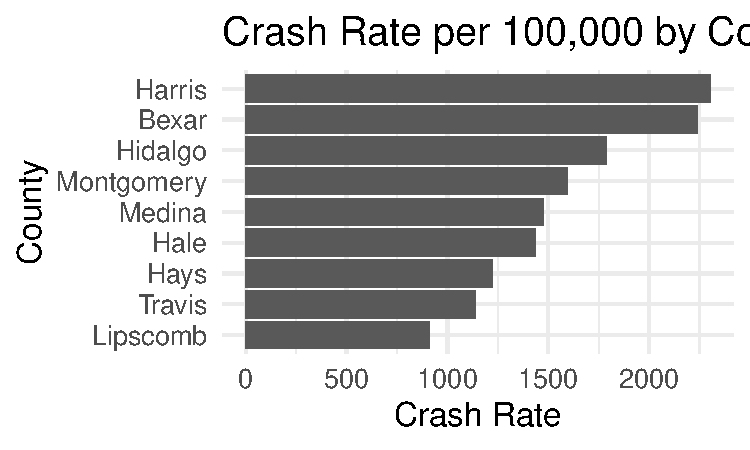
\includegraphics{senior_project_slides_v1_files/figure-beamer/unnamed-chunk-1-1} \end{center}
\end{frame}

\begin{frame}{Does Harris Have the Worst Drivers?}
\phantomsection\label{does-harris-have-the-worst-drivers}
\begin{itemize}
\tightlist
\item
  Harris County has the highest crash rate
\item
  However:

  \begin{itemize}
  \tightlist
  \item
    difference from Bexar is small
  \item
    not dramatically worse than other large counties
  \end{itemize}
\end{itemize}

\begin{block}{Conclusion}
\phantomsection\label{conclusion}
Houston is not overwhelmingly worse, just slightly higher.
\end{block}
\end{frame}

\begin{frame}{Ranking Counties by Fatal Crash Rate}
\phantomsection\label{ranking-counties-by-fatal-crash-rate}
\begin{longtable}[]{@{}lrrr@{}}
\caption{Counties ranked by fatal crash rate per 100,000}\tabularnewline
\toprule\noalign{}
County & Fatal\_Rate & Fatal\_Crashes & Population \\
\midrule\noalign{}
\endfirsthead
\toprule\noalign{}
County & Fatal\_Rate & Fatal\_Crashes & Population \\
\midrule\noalign{}
\endhead
Lipscomb & 36.43 & 1 & 2745 \\
Medina & 19.42 & 11 & 56647 \\
Hale & 12.58 & 4 & 31802 \\
Harris & 10.91 & 546 & 5003892 \\
Travis & 9.96 & 139 & 1395906 \\
Bexar & 9.46 & 205 & 2167567 \\
Hays & 8.82 & 26 & 294840 \\
Montgomery & 7.61 & 59 & 775723 \\
Hidalgo & 6.14 & 57 & 928384 \\
\bottomrule\noalign{}
\end{longtable}

\begin{block}{Brief interpretation}
\phantomsection\label{brief-interpretation}
Fatal crash rate focuses on severity rather than frequency, so it can
highlight counties where crashes are less common but more dangerous.
\end{block}
\end{frame}

\begin{frame}{Risk Factor Table}
\phantomsection\label{risk-factor-table}
\begin{longtable}[]{@{}
  >{\raggedright\arraybackslash}p{(\linewidth - 8\tabcolsep) * \real{0.1594}}
  >{\raggedleft\arraybackslash}p{(\linewidth - 8\tabcolsep) * \real{0.1884}}
  >{\raggedleft\arraybackslash}p{(\linewidth - 8\tabcolsep) * \real{0.1594}}
  >{\raggedleft\arraybackslash}p{(\linewidth - 8\tabcolsep) * \real{0.2609}}
  >{\raggedleft\arraybackslash}p{(\linewidth - 8\tabcolsep) * \real{0.2319}}@{}}
\caption{Risk-factor proportions by county}\tabularnewline
\toprule\noalign{}
\begin{minipage}[b]{\linewidth}\raggedright
County
\end{minipage} & \begin{minipage}[b]{\linewidth}\raggedleft
SpeedPercent
\end{minipage} & \begin{minipage}[b]{\linewidth}\raggedleft
DUIPercent
\end{minipage} & \begin{minipage}[b]{\linewidth}\raggedleft
DistractedPercent
\end{minipage} & \begin{minipage}[b]{\linewidth}\raggedleft
SeverityPercent
\end{minipage} \\
\midrule\noalign{}
\endfirsthead
\toprule\noalign{}
\begin{minipage}[b]{\linewidth}\raggedright
County
\end{minipage} & \begin{minipage}[b]{\linewidth}\raggedleft
SpeedPercent
\end{minipage} & \begin{minipage}[b]{\linewidth}\raggedleft
DUIPercent
\end{minipage} & \begin{minipage}[b]{\linewidth}\raggedleft
DistractedPercent
\end{minipage} & \begin{minipage}[b]{\linewidth}\raggedleft
SeverityPercent
\end{minipage} \\
\midrule\noalign{}
\endhead
Montgomery & 0.3705 & 0.0393 & 0.1459 & 0.0291 \\
Hidalgo & 0.3359 & 0.0453 & 0.0947 & 0.0211 \\
Harris & 0.3240 & 0.0291 & 0.0855 & 0.2503 \\
Hays & 0.3115 & 0.0666 & 0.2526 & 0.0455 \\
Hale & 0.2735 & 0.0547 & 0.2363 & 0.0416 \\
Medina & 0.2344 & 0.0550 & 0.2285 & 0.0514 \\
Lipscomb & 0.2000 & 0.0000 & 0.0800 & 0.0400 \\
Travis & 0.1920 & 0.0745 & 0.3235 & 0.0410 \\
Bexar & 0.1549 & 0.0341 & 0.3660 & 0.0202 \\
\bottomrule\noalign{}
\end{longtable}
\end{frame}

\begin{frame}{Driving Behavior Across Counties}
\phantomsection\label{driving-behavior-across-counties}
\begin{itemize}
\tightlist
\item
  Speed-related crashes:

  \begin{itemize}
  \tightlist
  \item
    moderate across most counties
  \end{itemize}
\item
  DUI crashes:

  \begin{itemize}
  \tightlist
  \item
    relatively low percentages
  \end{itemize}
\item
  Distracted driving:

  \begin{itemize}
  \tightlist
  \item
    high in multiple counties, especially urban counties
  \end{itemize}
\end{itemize}

\begin{block}{Insight}
\phantomsection\label{insight}
Risk behaviors vary, but no single factor dominates.
\end{block}
\end{frame}

\begin{frame}{Speeding vs Crash Rate}
\phantomsection\label{speeding-vs-crash-rate}
\begin{center}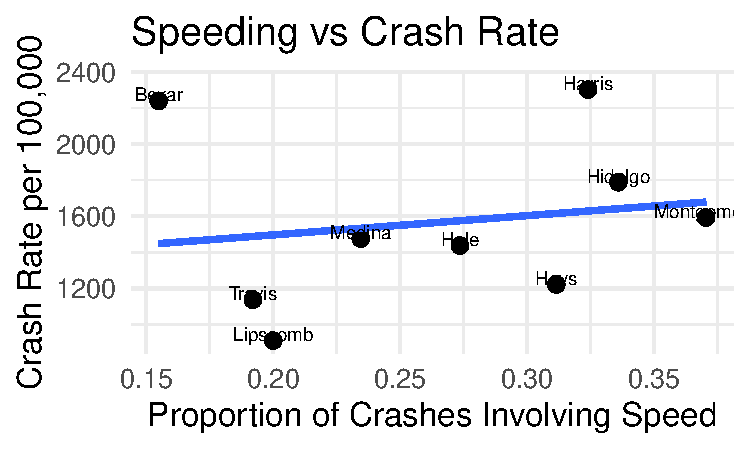
\includegraphics{senior_project_slides_v1_files/figure-beamer/unnamed-chunk-2-1} \end{center}

\begin{block}{Brief interpretation}
\phantomsection\label{brief-interpretation-1}
An upward trend would suggest that counties with more speed-related
crashes also tend to have higher crash rates.
\end{block}
\end{frame}

\begin{frame}{Distracted Driving vs Crash Rate}
\phantomsection\label{distracted-driving-vs-crash-rate}
\begin{center}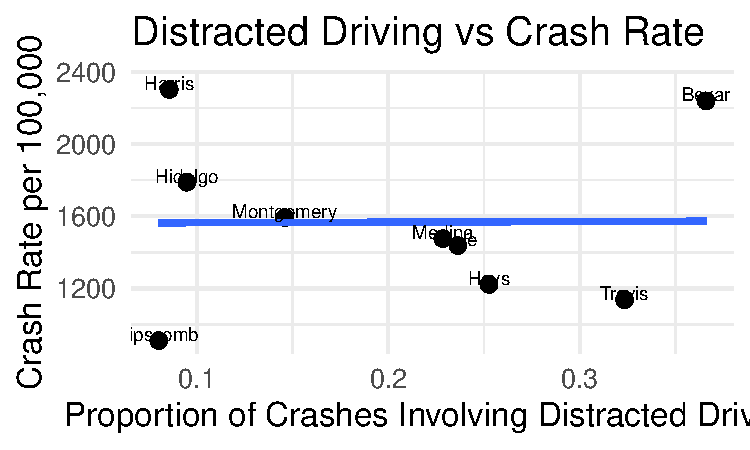
\includegraphics{senior_project_slides_v1_files/figure-beamer/unnamed-chunk-3-1} \end{center}

\begin{block}{Brief interpretation}
\phantomsection\label{brief-interpretation-2}
This plot checks whether distracted driving is associated with higher
crash rates across the sample counties.
\end{block}
\end{frame}

\begin{frame}{Confidence Intervals for County Crash Rates}
\phantomsection\label{confidence-intervals-for-county-crash-rates}
To estimate the true crash rate for each county, I used a 95\%
confidence interval.

\[
\hat{p}=\frac{\text{Total Crashes}}{\text{Population}}
\]

\[
\hat{p}\pm 1.96\sqrt{\frac{\hat{p}(1-\hat{p})}{n}}
\]

where:

\begin{itemize}
\tightlist
\item
  \(\hat{p}\) = observed crash proportion
\item
  \(n\) = county population
\item
  \(1.96\) gives a 95\% confidence level
\end{itemize}

\begin{block}{Purpose}
\phantomsection\label{purpose}
This helps show whether differences in county crash rates are likely to
be meaningful or just due to random variation.
\end{block}
\end{frame}

\begin{frame}{95\% Confidence Intervals by County}
\phantomsection\label{confidence-intervals-by-county}
\textbackslash begin\{table\}

\textbackslash caption\{\label{tab:ci-all-table}Crash rates and 95\%
confidence intervals per 100,000 residents\} \centering

\begin{tabular}[t]{lrrr}
\toprule
County & Crash\_Rate & Lower\_CI & Upper\_CI\\
\midrule
Harris & 2301.67 & 2288.53 & 2314.81\\
Travis & 1137.04 & 1119.45 & 1154.63\\
Bexar & 2238.55 & 2218.85 & 2258.24\\
Montgomery & 1592.32 & 1564.46 & 1620.18\\
Hays & 1221.68 & 1182.03 & 1261.33\\
\addlinespace
Medina & 1475.81 & 1376.51 & 1575.11\\
Hidalgo & 1788.16 & 1761.20 & 1815.12\\
Hale & 1437.02 & 1306.21 & 1567.82\\
Lipscomb & 910.75 & 555.36 & 1266.13\\
\bottomrule
\end{tabular}

\textbackslash end\{table\}
\end{frame}

\begin{frame}{Crash Rates with 95\% Confidence Intervals}
\phantomsection\label{crash-rates-with-95-confidence-intervals}
\begin{center}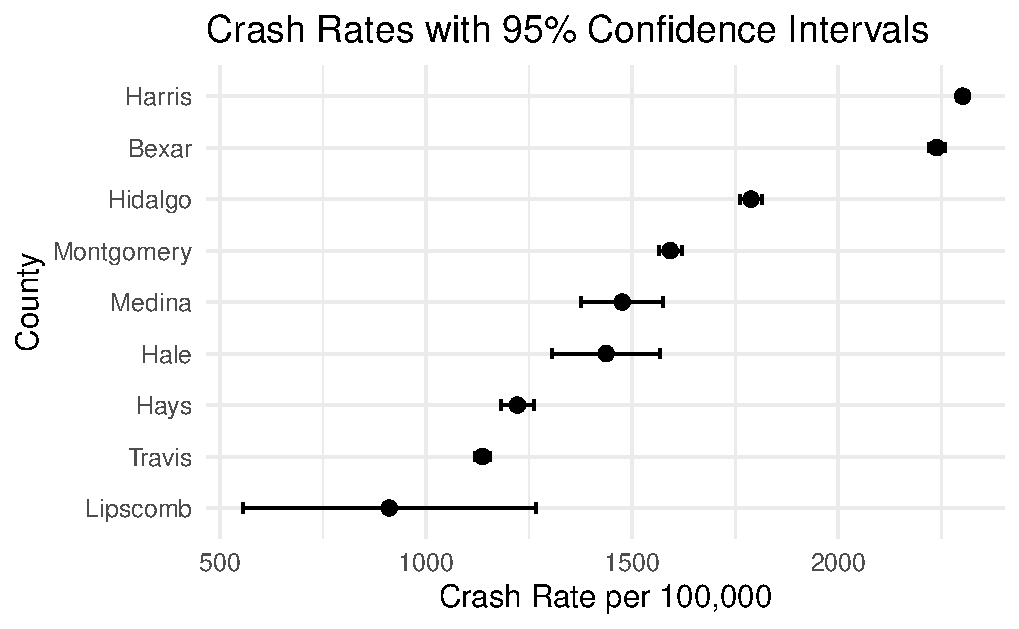
\includegraphics{senior_project_slides_v1_files/figure-beamer/ci-all-plot-1} \end{center}
\end{frame}

\begin{frame}{Interpreting the Confidence Intervals}
\phantomsection\label{interpreting-the-confidence-intervals}
\begin{itemize}
\tightlist
\item
  If two counties have intervals that do not overlap, that suggests
  stronger evidence that their crash rates are different
\item
  If two counties have intervals that overlap a lot, then the difference
  may not be statistically meaningful
\end{itemize}

\begin{block}{Harris vs Montgomery}
\phantomsection\label{harris-vs-montgomery}
\begin{itemize}
\tightlist
\item
  Harris County has a higher observed crash rate than Montgomery County
\item
  But if their intervals overlap, then the data does not clearly show
  that Harris is worse
\item
  This matters because neighboring counties may share highways, commuter
  traffic, and similar driving environments
\end{itemize}
\end{block}

\begin{block}{Main Point}
\phantomsection\label{main-point}
Confidence intervals help move the project beyond simple ranking and
toward statistical comparison.
\end{block}
\end{frame}

\begin{frame}{Regression Model}
\phantomsection\label{regression-model}
\[
\text{Crash Rate}=\beta_0+\beta_1(\text{SpeedPercent})+\beta_2(\text{DUIPercent})+\beta_3(\text{DistractedPercent})+\varepsilon
\]

\begin{itemize}
\tightlist
\item
  Goal: identify which behaviors increase crash rates
\end{itemize}
\end{frame}

\begin{frame}{Are the results significant?}
\phantomsection\label{are-the-results-significant}
\begin{longtable}[]{@{}lrrrr@{}}
\caption{Regression coefficients}\tabularnewline
\toprule\noalign{}
term & estimate & std.error & statistic & p.value \\
\midrule\noalign{}
\endfirsthead
\toprule\noalign{}
term & estimate & std.error & statistic & p.value \\
\midrule\noalign{}
\endhead
(Intercept) & 84.007 & 1372.552 & 0.0612 & 0.9536 \\
SpeedPercent & 5107.916 & 4239.003 & 1.2050 & 0.2821 \\
DUIPercent & -16501.027 & 14148.702 & -1.1663 & 0.2961 \\
DistractedPercent & 4237.233 & 3694.462 & 1.1469 & 0.3033 \\
\bottomrule\noalign{}
\end{longtable}

\begin{itemize}
\tightlist
\item
  All p-values \textgreater{} 0.05
\item
  None of the variables are statistically significant
\end{itemize}

\begin{block}{Interpretation}
\phantomsection\label{interpretation}
We cannot confidently say any factor causes higher crash rates.
\end{block}
\end{frame}

\begin{frame}{Regression Findings}
\phantomsection\label{regression-findings}
\begin{longtable}[]{@{}rrrrr@{}}
\caption{Regression model fit}\tabularnewline
\toprule\noalign{}
r.squared & adj.r.squared & sigma & statistic & p.value \\
\midrule\noalign{}
\endfirsthead
\toprule\noalign{}
r.squared & adj.r.squared & sigma & statistic & p.value \\
\midrule\noalign{}
\endhead
0.25 & -0.2 & 519.6527 & 0.5556 & 0.6667 \\
\bottomrule\noalign{}
\end{longtable}

\begin{itemize}
\tightlist
\item
  \(R^2 = 0.25\)
\item
  Model explains only about 25\% of the variation
\end{itemize}

\begin{block}{Coefficients}
\phantomsection\label{coefficients}
\begin{itemize}
\tightlist
\item
  Speed → positive effect
\item
  Distracted → positive effect
\item
  DUI → unclear or negative effect
\end{itemize}
\end{block}
\end{frame}

\begin{frame}{Interpretation of Results}
\phantomsection\label{interpretation-of-results}
Crash rates are not fully explained by:

\begin{itemize}
\tightlist
\item
  Speed
\item
  DUI
\item
  Distracted driving
\end{itemize}

\begin{block}{Likely Explanation}
\phantomsection\label{likely-explanation}
Other factors may matter more:

\begin{itemize}
\tightlist
\item
  Traffic density
\item
  Urban congestion
\item
  Road design
\end{itemize}
\end{block}
\end{frame}

\begin{frame}{Limitations}
\phantomsection\label{limitations}
\begin{itemize}
\tightlist
\item
  Small sample size (\(n = 9\) counties)
\item
  Limited variables
\item
  Regression results are not statistically significant
\end{itemize}

\begin{block}{Implication}
\phantomsection\label{implication}
The results suggest trends, but not definitive causation.
\end{block}
\end{frame}

\begin{frame}{Final Conclusion}
\phantomsection\label{final-conclusion}
\begin{itemize}
\tightlist
\item
  Harris County has the highest crash rate
\item
  But:

  \begin{itemize}
  \tightlist
  \item
    only slightly higher than Bexar
  \item
    not strongly explained by driver behavior
  \end{itemize}
\end{itemize}

\begin{block}{Final Answer}
\phantomsection\label{final-answer}
Harris does not clearly have the ``worst drivers.''
\end{block}
\end{frame}

\end{document}
